\chapter{Numerical Background}
%\begin{itemize}
%\item introduction to the boussinesq approximation 
%\item In this section I should introduce the spectral method and the numerical scheme
%\item Dealiasing tests 
%\item  diffusion test
%\item hyperviscosity
%\end{itemize}

In this chapter we discuss the numerical techniques and methods used in this thesis. In this thesis we use the spectral method to numerically solve the Navier-Stokes equations. Spectral methods provide a convenient and quick way to compute derivatives of sufficiently well-behaved periodic functions. In evaluating derivatives of smooth periodic functions, spectral methods provide an advantage over other methods of evaluating derivatives, such as finite difference, as the derivatives can be computed to much great accuracy, often 10 digits, in exchange for only a relatively modest increase in complexity. Specifically, finite difference methods run in $\mathcal{O}(N)$ but the error tends to be on the order of $\mathcal{O}(N^{-1})$ while spectral methods run in $\mathcal{O}(n\log n)$ but the errors are on the order of $\mathcal{O}(N^{-p})$ when the function is $C^{p}$. A complete overview of spectral methods is beyond the scope of this thesis and we only discuss the key features needed for numerical work. Comprehensive reviews of spectral methods are provided in many books, e.g. Trefethen \cite{trefethen_spectral}, Boyd \cite{boyd2001}, and (spectral method in fluids book). 


\section{Spectral Methods Motivation}
Spectral methods have their origins in the Fourier transform. Let us denote the Fourier transform, $\mathcal{F}$, of $f(x)$ as $\mathcal{F}(f(x)) = \hat{f}(k)$, given by
\begin{align}
\mathcal{F}(f(x)) = \hat{f}(k) = \int_{-\infty}^{\infty}dxe^{-ikx}f(x)\label{fouriertransform}
\end{align}
Now consider the Fourier transform of the derivative $df/dx$. 
\begin{align}
\mathcal{F}\left(\frac{df}{dx}\right)= \int_{-\infty}^{\infty}dxe^{-ikx}\frac{df}{dx}=e^{-ikx}f(x)\bigg|_{-\infty}^{\infty} + ik\int_{-\infty}^{\infty}dxe^{-ikx}f(x)= ik\hat{f}(k)
\end{align}
and thus the Fourier transform of a derivative is just $ik$ times the Fourier transform of $f(x)$. An important assumption here that $f(x)$ vanishes sufficiently quickly at infinity otherwise the $e^{-ikx}f(x)$ term is non-negligible. For most applications of the Fourier transform, but not all,  this assumption is valid. In this thesis, all functions considered will vanish sufficiently so that this term is negligible. For a rigorous treatment of when this situation occurs, consult any book on Fourier methods. With this result in hand, it is easy to show via induction that the Fourier transform of $d^{n}f/dx^{n}$ is $(ik)^{n}\hat{f}(k)$. Hence, once we have the Fourier transform $\hat{f}(k)$, the $n$-th derivative is obtained by computing the inverse Fourier transform
\begin{align}
\frac{d^{n}f}{dx^{n}} = \frac{1}{2\pi} \int_{-\infty}^{\infty}dx e^{ikx}(ik)^{n}\hat{f}(k)
\end{align}

Computationally, if we have a quick way to evaluate $\hat{f}(k)$ from $f(x)$ and $f(x)$ from $\hat{f}(k)$, then the $n$th derivative is easy to compute: compute $\hat{f}(k)$, multiply by $(ik)^{n}$, invert $(ik)^{n}\hat{f}(k)$. The operation to quickly compute the Fourier transform is called, rather unsurprisingly, the fast Fourier transform, also commonly known as the FFT. 

\section{FFT and Spectral Derivatives} 
More discussion on the FFT here. Basic definition. Some examples of spectral differentiation from Trefethen.

Let us now investigate how we can quickly compute the Fourier transform. In analogue to the Fourier transform, we define the discrete Fourier transform\footnote{Note that there is no universal standard on where to put the factors of $N$ and $2\pi$.}
\begin{align}
\hat{v}_{k} = \frac{2\pi}{N}\sum_{j=1}^{N} e^{-ikx_{j}}v_{j},\qquad k=-\frac{N}{2}+1,\ldots,\frac{N}{2}
\end{align}
and the inverse Fourier transform 
\begin{align}
v_{j} = \frac{1}{2\pi}\sum_{k=-N/2+1}^{N/2} e^{ikx_{j}}\hat{v}_{k}, \qquad j=1,\ldots, N
\end{align}
Note that the range of the wavenumbers is from $-N/2+1$ not $-N/2$ due to the $2\pi$ periodicity so wavenumbers $-N/2$ are equivalent to $N/2$ and we do not want to count this wavenuber twice. 

From the definitions of the DFT and inverse DFT, we can see a close analogy to the continuous Fourier and inverse Fourier transforms. Analogously, it can be shown \cite{trefethen_spectral} that these are the correct discrete analogies. Thus if $v_{j}$ are the samples of some function, by compute the DCT $\hat{v}_{k}$, multiplying by $ik$ and computing the inverse DFT will produce the derivative of the sampled function $v'_{j}$. However, there is some subtleness involved in treating the wavenumber $N/2$, but to make a long story short, we simply set it to $0$ and for details see \cite{trefethen_spectral}.  

Our goal has still not been reached because we are still left with computer $\mathcal{O}(N^{2})$ terms. This is where the development of the FFT comes into play.  

The algorithm to compute the FFT is a divide and conquer algorithm. The basic idea is to notice that computing the discrete Fourier transform can be divided into even and odd terms. From there, which can be computed independently of each other. Thus assuming $N$ is a power of two, we have two new discrete Fourier transform problems of size $N/2$. Each other those problems can themselves be decomposed into problems of size $N/4$. Repeating this process recursively we are able to divide the computation of the DFT into $\mathcal{O}(\log N)$ problems. Computing the DFT of each problem takes roughly $\mathcal{O}(N)$ and thus the total running time is on the order of $\mathcal{O}(N\log N)$. This is only a brief overview of the result for the case of $N$ being a power of two. In this simple case, it is easy to prove rigorously from the recursion relationship that the running time is $\mathcal{O}(N\log N)$ using the Master theorem (cite CLRS). 

The derivation and implementation of the FFT for general values of $N$ is an interesting and complicated question that has sparked a lot of research into the best way to decompose the problem. Additionally, the actual implementation details can differ depending on the value of $N$, the type of computer, and the type of data being considered. It is beyond the scope of the thesis to discuss any sorts of details and further details technical and hardware details can be found in (cite that FFT implementation book) and implementation details can be found in (cite FFTW manual).

For example, we follow \cite{trefethen_spectral} and demonstrate spectral differentiation using two simple examples to illustrate spectral methods. Consider the following two periodic functions
\begin{align}
f(x) = \max(0,1-|x-\pi|/2), \qquad g(x)=e^{\sin x}
\end{align}
which are both periodic on the interval $[0,2\pi]$.  Figure goes here. 

As we can see, when the original function is sufficiently smooth and periodic, here $g(x)$, the accuracy of the derivative is very good. However, when the function is not smooth, as exhibited in $f(x)$, the accuracy is not very good. Here $g(x)$ is not differentiable at $\pi$ and spectral methods have a difficult time dealing with this. For a complete discussion of the specific smoothness and accuracy is contained in Chapter 4 of \cite{trefethen_spectral}.
\section{Dealiasing} 
In the previous section we demonstrated that spectral differentiation can produce very accurate results in only $\mathcal{O}(N\log N)$ operations. However, we have only considered the spectral derivative of a single function $f(x)$, the question naturally arises about what happens if we have more general expressions, for example advection like terms in the Navier-Stokes equations 
\begin{align}
u\frac{\partial u}{\partial x} + v\frac{\partial u}{\partial y} +w\frac{\partial u}{\partial z}
\end{align}
where we now have a product of a function and a derivative. Such terms are known as a convolution and require a more careful treatment. In this section, we introduce two closely related methods for evaluating expressions of the above form, the spectral method and the pseudospectral method. For this we carefully follow the treatment of Durran \cite{durran}. 

Consider the following general 1D non-linear PDE
\begin{align}
\frac{\partial \psi}{\partial t} + F(\psi) = 0
\end{align}
where $F(\psi)$ is some general nonlinear function. Consider seeking a series expansion of the form
\begin{align}
\psi(x,t)\approx \phi(x,t) = \sum_{k=1}^{N}a_{k}(t)\varphi_{k}(x)
\end{align}
where $\varphi_{k}$ is some basis function that we are interested in expanding the solution in. Some examples of such functions might be complex exponentials, Bessel functions, or spherical harmonics, however, in general,  we will not be able to find the eigenfunctions that provide the natural basis to seek a series expansion. Without the proper basis functions, it is clear that the approximate solution will never exactly solve the original PDE and we have to determine a way to minimise the error. For many problems, there is often some degree of symmetry so choosing a certain basis makes sense. For example, a problem within a box, it makes sense to choose complex exponentials as a base or if the problem is based on a sphere, spherical harmonics are a natural choice. Thus, we are interested in not finding the correct $\varphi_{k}$ but instead focus picking a basis and appropriately choosing $a_{k}(t)$ to minimise the residual, 
\begin{align}
R(\phi) = \frac{\partial \phi}{\partial t} + F(\phi),
\end{align}
in some way.  

How we choose to evaluate this error leads to different methods of solving the problem. Right now we consider the so-called "spectral method" which is a special case of a very general technique called Galerkin approximation.  The spectral method requires the residual be orthogonal to the basis functions $\varphi_{k}$, i.e.
\begin{align}
\int_{S}R(\phi(x))\varphi_{k}(x)dx = 0 \qquad k=1,\ldots,N.
\end{align}
For the special case of the spectral method, we require that the basis functions be orthogonal. If this restriction is relaxed the resulting method is known as the finite element method. 

By requiring the above integral to be minimised, it can be shown\cite{durran} that the resulting system of ODEs for the above is
\begin{align}
\frac{d a_{k}}{dt} = -\frac{1}{M_{k,k}}\int_{S}\left[F\left(\sum_{n=1}^{N}a_{n}\varphi_{n}\right)\varphi_{k}\right]dx \qquad k=1,\ldots,N
\end{align}
where $M_{k,k}=\langle \varphi_{k},\varphi_{k}\rangle$. For our work, we are interested in a specific case of basis functions, $\varphi_{k}(x)=e^{ikx}$ and the inner product to be the standard inner product for complex functions
\begin{align}
\int_{S}g(x)h^{*}(x)dx=0 
\end{align}

Using the above, let use the spectral method to solve the 1D advection equation with variable windspeed,
\begin{align}
\frac{\partial\phi}{\partial t} + c(x,t)\frac{\partial \phi}{\partial x} =0, F(\phi) = c(x,t)\frac{\partial \phi}{\partial x}
\end{align}
Let us expand out $\phi(x,t)$ as the sum of $N=2K+1$ Fourier modes
\begin{align}
\phi(x_{j},t)= \sum_{n=K}^{K}a_{n}(t)e^{inx_{j}}
\end{align}
plugging this into the above yields
\begin{align}
\frac{d a_{k}}{dt} = -\frac{i}{2\pi}\sum_{n=-K}^{K}na_{n}\int_{-\pi}^{\pi}c(x,t)e^{i(n-k)x}dx \qquad k=-K,\ldots,K
\end{align}
Expanding out $c(x,t)$ as a Fourier series we obtain
\begin{align} 
\frac{d a_{k}}{dt} = -\frac{i}{2\pi}\sum_{n=-K}^{K}\sum_{m=-K}^{K}na_{n}c_{m}\int_{-\pi}^{\pi}e^{i(n+m-k)x}dx \qquad k=-K,\ldots,K
\end{align}
and upon using the orthogonality of the integral, we obtain
\begin{align}
\frac{da_{k}}{dt} = -\sum_{\substack{m+n=k\\ |m|,|n|\le K}} inc_{m}a_{n}
\end{align}
where we require that $n+m=k$ and $|n|,|m|\le K$. If we want to evaluated this sum directly, we would need to evaluate $\mathcal{O}(K^{2})$ operations due to the double sum required to evaluate the convolution. Historically, this was a barrier for spectral methods because even though they provided accurate results, this $\mathcal{O}(K^{2})$ bottleneck did not allow for larger numerical simulations, where $\mathcal{O}(K)$ finite differences method could. (ref)

In order to get around this bottleneck, we can turn the $\mathcal{O}(K^{2})$ to $\mathcal{O}(K\log K)$, however we do this at the cost of additional processing. The general idea is as follows: transform the Fourier coefficients to real space in $\mathcal{O}(K\log K)$, multiply the two terms together at each grid point in $\mathcal{O}(K)$, and transform back to Fourier space in $\mathcal{O}(K\log K)$. The resulting algorithm is $\mathcal{O}(K\log K)$. However, if we were to implement this naively, errors would arise, due to the phenomena of aliasing. 

Aliasing is an effect that is common. An exaggerated example, known as the wagon wheel effect (Wikipedia) is when an object appears to be stationary but is really moving. For example, imagine a camera that takes a picture every second of a turbine, but the turbine is moving at 10 revolutions per second. For someone looking at the shots from the camera, they would claim the turbine isn't moving. If the turbine is moving slightly faster, say 10.1 revolutions per second, the camera would show that the turbine is moving, albeit rather slowly. If it were moving slightly slower, say 9.9 revolutions per second, the camera would show the turbine moving backwards.


\begin{figure}
\begin{center}
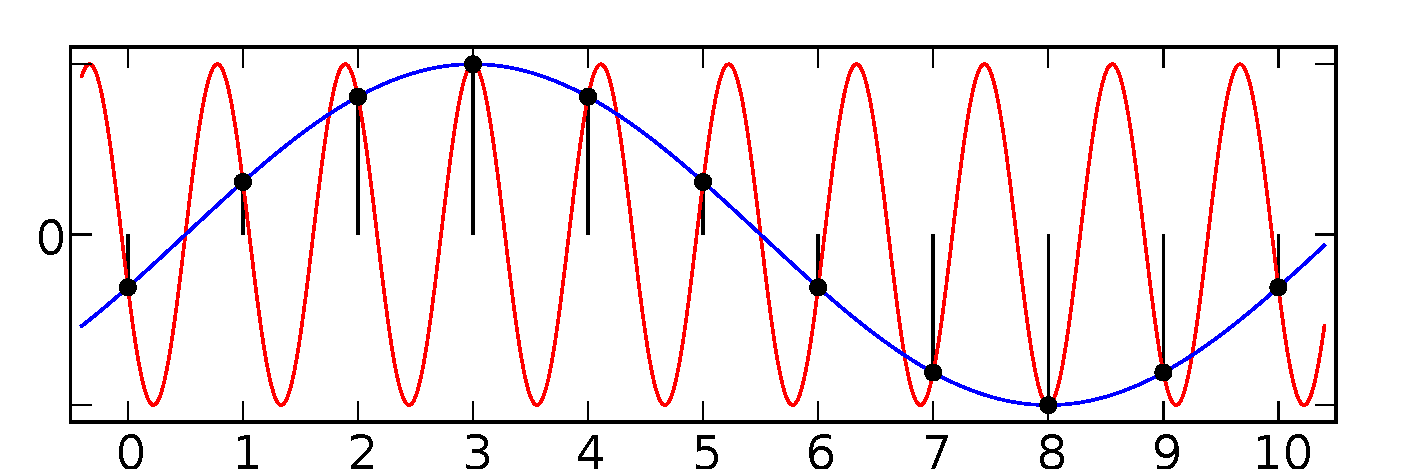
\includegraphics[width=\textwidth]{aliassine.pdf}
\caption{Different sine curves that fit the same set of data points. This is an example of aliasing. Source http://en.wikipedia.org/wiki/File:AliasingSines.svg}
\end{center}
\label{aliassine}
\end{figure}
Mathematically, we can see a similar phenomena by sampling a sine wave. Consider Figure~\ref{aliassine} which has 11 points. The short wavelength red sine curve samples these points with a short wavelength while a longer wavelength blue curve also samples, despite being non-existent in the actual data. The goal is to minimise this effect. 

To illustrate this consider two functions $f(x),g(x)$ and we want to compute the Fourier coefficients so that
\begin{align}
f(x)g(x) = \sum_{m=-K}^{K} p_{k}e^{ikx}
\end{align}
and we can expand $f(x),g(x)$ as Fourier series
\begin{align}
f(x) = \sum_{m=-K}^{K}a_{m}e^{imx}, \qquad g(x) = \sum_{n=-K}^{K}b_{n}e^{inx}
\end{align}
The above algorithm states that we convert the Fourier coefficients $a_{m},b_{n}$ to real space and multiply. Suppose that in real space the spacing between the grid points is
\begin{align}
x_{j} = \frac{2\pi j}{2N+1}
\end{align}
however how do we choose $N$? Naively, it seems logical to set that $N=K$ so that both real and Fourier space have the same number of co-efficients. This naive choice leads to aliasing error and instead we must choose $N>K$ to avoid this aliasing error. To get intuition for why, aliasing error arises when two poorly resolved waves are multiplied together and produce a longer wavelength wave, as discussed above in Figure~\ref{aliassine}. We can avoid this if all short wavelengths are resolved properly. (insert figure 6.2 Durran).

To find the optimal value of $N$, consider the case in Figure. When we multiply two short wavelengths, we choose two large values of $k$, recalling that large $k$ is short wavelengths and small $k$ are long wavelengths. Also recall that multiplication of waves is addition of wavenumbers. Thus the resulting wavenumber is $\tilde{k}= k_{1}+k_{2}-2\pi/\Delta x_{e}$. We want to choose $\pi/\Delta x_{e}$ so that all the potential wavenumbers fall within the range $-K\le k\le K$. The largest potential case is when $k_{1,2}=K$ so we require that
\begin{align}
K<|2K- \frac{2\pi}{\Delta x_{e}}|
\end{align}
and upon subbing in $\Delta x_{e}$ we find that 
\begin{align}
N > \frac{3}{2}K - 1
\end{align}
(add in grindy algebra one).

A closely related, but different method is known as, somewhat confusingly, as the pseudospectral method.  In this case, instead of enforcing that the residual is orthogonal to the basis functions, we instead choose a collocation method, i.e.
\begin{align}
R(\phi(k\dx)) = 0 \qquad k=1,\ldots,N
\end{align}
Here, upon substituting in the $\phi(x,t)$ and $c(x,t)$ we find that
\begin{align}
\frac{d\phi_{j}}{dt} + c_{j}\frac{\partial \phi_{j}}{\partial x} = 0
\end{align}
(add in a lot of the algebra)

It is important to realise that the spectral and pseudospectral method are two very different approaches that yield very similar algorithms to solving the same problem. Both make use of the FFT as a convenient and quick way to evaluate derivatives. In a sense, the pseudospectral method is the spectral method with no dealiasing on evaluating the convolution sum. To illustrate this, consider solving the viscous Burger's equation
\begin{align}
\frac{\partial \phi}{\partial t} + \phi\frac{\partial \phi}{\partial x} = \nu \frac{\partial^{2}\phi}{\partial x^{2}}
\end{align}
with a Gaussian initial condition. We solve the above with an RK4 scheme, but the important thing is the energy. See Figure. 

%In Panel A we have spectral methods and we can see that the total energy is constant while with the pseudospectral in Panel B diverges. 

Discuss dealiasing of linear and nonlinear code as well. Show plots. 
\section{Timestepping and Examples}
More complete discussion of time-stepping to be included. 

In this section we demonstrate the differences between solving PDEs in real space vs Fourier space. Consider the following one dimensional wave equation\cite{trefethen_spectral}
\begin{align}
\frac{\partial u}{\partial t} + c(x)\frac{\partial u}{\partial x} = 0,\qquad c(x)=\frac{1}{5}+\sin^{2}(x-1), \qquad u(x,0)=e^{-100(x-1)^{2}}, x\in[0,2\pi], t>0
\end{align}
where we are solving on a periodic domain. The physical interpretation of this equation is the simple one dimensional advection of a velocity field $u(x,t)$ by the fixed field $c(x)$. To evaluate the advection term, we use a spectral method with 2/3s dealiasing. As discussed in the previous section, there is still non-standard terminology throughout the literature regrading the names of the various methods of using FFTs. Trefethen, for example, calls pseudospectral methods, 'collocation methods'. 

For a time-stepping scheme, we use a second-order Adams-Bashforth\cite{durran} scheme. Re-writing wave-equation as
\begin{align}
\frac{\partial u}{\partial t} = -c(x)\frac{\partial u}{\partial x} = F(u)
\end{align}
the Adams-Bashforth scheme is
\begin{align}
u^{n+1} = u^{n} + \frac{\dt}{2}[3F(u^{n})-F(u^{n-1})]
\end{align}
Since the Adams-Bashforth scheme uses a previous time-step, we will use forward Euler for the first time-step. To evaluate $F(u)$ we will use the spectral differentiation, as discussed above. 
Figures go here.


Add 2D NS solver example??

\section{Navier-Stokes in Fourier Space}
\subsection{Fourier Transformed Navier-Stokes}
We now turn to the formulation of the Navier-Stokes equations in a Fourier domain. The Fourier domain provides a convenient formulation to analyse the underlying mechanisms of turbulence, as we shall see. Recall that in the Fourier domain, derivatives become multiplication of wavenumbers which converts the spatial parts of the Navier-Stokes equations into algebraic equations. 

To demonstrate the formulation in Fourier space, let us cast the standard Navier-Stokes equations into Fourier space. 
\begin{align}
\frac{\partial \textbf{u}}{\partial t} + \textbf{u}\cdot\nabla\textbf{u} = -\frac{1}{\rho_{0}}\nabla p + \nu\nabla^{2}\textbf{u}, \qquad \nabla\cdot\textbf{u}=0
\end{align}
Taking the Fourier transform of the above equation is straight-forward for all terms except the advection term $\textbf{u}\cdot\nabla\textbf{u}$, which we postpone for now.

In Fourier space, we can also exploit the following observation to eliminate the pressure term, thus saving the need to solve a Poisson equation at each time-step. The incompressibility condition becomes $\textbf{k}\cdot\hat{\textbf{u}}(\textbf{k},t)=0$ in Fourier space. Geometrically, this means that the vectors $\textbf{k}$ and $\hat{\textbf{u}}$ are orthogonal. To see this define a $\textbf{k}$-plane and a $\hat{\textbf{u}}$-plane. The defining equation of a plane is $ax+by+cz=d$ with the normal vector $\textbf{n}=(a,b,c)$. Here the normal vectors are $\textbf{k}$ and $\hat{\textbf{u}}$. Thus if the normal vectors are orthogonal, the planes are orthogonal.

This realisation tells us that vectors that are proportional to \uhatm are orthogonal to vectors that are proportional to \kvecm. Thus writing out the Navier-Stokes equations
\begin{align}
\frac{\partial \uhat}{\partial t} + \mathcal{F}(\textbf{u}\cdot\nabla\textbf{u}) = -\frac{1}{\rho_{0}} \kvec\hat{p} - \nu k^{2}\uhat\label{NS_fourier_1},
\end{align}
take the dot product with \kvecm and using the orthogonality condition we obtain
\begin{align}
\kvec\cdot\mathcal{F}(\textbf{u}\cdot\nabla\textbf{u}) + \frac{1}{\rho_{0}}k^{2}\hat{p}=0\label{pressure_fourier_1}.
\end{align}
Isolating for pressure and substituting back into (\ref{NS_fourier_1}) we obtain
\begin{align}
\frac{\partial \uhat}{\partial t} + \mathcal{F}(\textbf{u}\cdot\nabla\textbf{u})(\textbf{1}-\frac{\kvec\kvec}{k^{2}})= - \nu k^{2}\uhat\label{NS_fourier_2}.
\end{align}
This result is unsurprising, since all we have done is take the divergence of the Navier-Stokes equations, which in Fourier space corresponds to taking the dot product with respect to $\kvec$. But using this observation we can avoid the need for solving the pressure altogether because the pressure term is orthogonal to the $\uhat$-plane. But what about the advection term? As can be seen in (\ref{NS_fourier_2}), it has this factor $\textbf{1} - \kvec\kvec/k^{2}$ multiplying it. This term represents a projection into the $\uhat$-plane. The advection term can thought of a vector that is pointing in some direction in-between the planes of $\kvec$ and $\uhat$. By projecting the advection term into the $\uhat$-plane, we would have a set of equations that are independent of the pressure completely.

\subsection{Projection Tensor}
In order to project the Navier-Stokes equations onto the $\uhat$-plane, we define the following projection operator
\begin{align}
\textbf{P}=\textbf{1} - \frac{\kvec\kvec}{k^{2}} = P_{ij}(\kvec) = \delta_{ij} - \frac{k_{i}k_{j}}{k^{2}}
\end{align}
where we are using Einstein summation notation \cite{lesieur,wald}. It is straight forward to verify that $P_{ij}P_{jk}=P_{ik}$ or in matrix notation $\textbf{P}^{2}=\textbf{P}$, in other words the projection tensor is idempotent. Idempotence is a defining feature of projection operators \cite{MeyerLinAlg}. It is straightforward to verify that $k_{j}P_{ij}=0$ and $\hat{u}_{j}P_{ij}=\hat{u}_{i}$. These simple observations confirm that the projection tensor projects a vector onto the $\uhat$-plane. 

Applying $P_{ij}$ to (\ref{NS_fourier_1}) we obtain the following 
\begin{align}
\frac{\partial \uhat}{\partial t} + \textbf{P}\mathcal{F}(\textbf{u}\cdot\nabla\textbf{u}) =  -\nu k^{2}\uhat\label{NS_fourier_3}
\end{align}
where $\textbf{P}$ is acting on the Fourier transform of the advection term. In order to compute the Fourier transform of the advection term, we note that 
\begin{align}
\textbf{u}\cdot\nabla\textbf{u} = u_{j}\frac{\partial u_{i}}{\partial x_{j}} = \frac{\partial (u_{i}u_{j})}{\partial x_{j}}
\end{align}
where the incompressibility condition has been used to bring the velocity inside the derivative. Thus we are able to write
\begin{align}
\mathcal{F}(\textbf{u}\cdot\nabla\textbf{u})=ik_{j}\int_{\textbf{p}+\textbf{q}=\kvec}d\kvec\hat{u}_{i}(\textbf{p})\hat{u}_{j}(\textbf{q})
\end{align}
and hence we can finally write out the Navier-Stokes equations in Fourier space as \cite{lesieur}
\begin{align}
\frac{\partial \hat{u}_{i}}{\partial t} + iP_{ij}k_{m}\int_{\textbf{p}+\textbf{q}=\kvec}d\kvec\hat{u}_{j}(\textbf{p})\hat{u}_{m}(\textbf{q})=  -k^{2}\hat{u}_{i}\label{NS_fourier_3}
\end{align}

\subsection{Numerical Formulation of NS in Fourier}
Although we have eliminated the pressure completely, we still have an integral term in the equation. To formulate this problem numerically, we make the following observation that is useful in spectral methods \cite{lesieur,orszag1972}.

Recall the following identity (Kundu, Acheson)
\begin{align}
\textbf{u}\cdot\nabla\textbf{u} = \bm{\omega}\times \textbf{u} - \frac{1}{2}\nabla \textbf{u}^{2}
\end{align}
When we apply the projection operator $\textbf{P}$ to the above equation, the $\nabla \textbf{u}^{2}$ term will vanish since it is orthogonal to the $\uhat$-plane. For the cross product between the vorticity and velocity, we use the methods discussed above from dealiasing. Thus to evaluate the cross product term, we assume we have the Fourier transform of the vorticity and velocity $\hat{\bm{\omega}},\uhat$ and re-write the cross product term as
\begin{align}
\mathcal{F}(\bm{\omega}\times \textbf{u}) = \mathcal{F}(\mathcal{F}^{-1}(\hat{\bm{\omega}})\times\mathcal{F}^{-1}(\uhat))
\end{align}
Using this result we can reformulate the Navier-Stokes equations into a form to be solved numerically using a spectral method
\begin{align}
\frac{\partial \uhat}{\partial t} = \textbf{P}(\kvec)\mathcal{F}(\mathcal{F}^{-1}(\hat{\bm{\omega}})\times\mathcal{F}^{-1}(\uhat))-k^{2}\uhat
\end{align}
where the $\mathcal{F},\mathcal{F}^{-1}$ can be evaluated by FFTs, as discussed above.

This reformulation of the Navier-Stokes equations into Fourier space simplifies numerical calculations immensely and provides many advantages over the real space formulation. The absence of the pressure term means that there is no Poisson equation to be solved at each time-step for the pressure. If one did want the pressure, one can solve (\ref{pressure_fourier_1}) for $\hat{p}$. In addition there is no need to enforce a divergence free solution\footnote{Except possibly at the initial time step, see Section 3.} as the equations are formulated by definition to satisfy divergence free condition. The only additional technical difficulty is evaluating the vorticity, but this can easily be handled because of the simple structure of the curl. 

\subsection{Integrating Factor}
Another advantage of the Fourier formulation is the ability to exactly integrate the diffusion term. Let us denote the advective projective term as $F(\hat{u})$ and we have
\begin{align}
\frac{\partial \uhat}{\partial t} + \nu k^{2}\uhat = F(\uhat) 
\end{align}
where the left-hand side has been explicitly written out. Written in this form, the common trick of writing a product as a derivative is observed since
\begin{align}
 \frac{\partial \uhat}{\partial t} + \nu k^{2}\uhat= e^{-\nu k^{2}t}\frac{\partial \uhat e^{\nu k^{2}t}}{\partial t} 
\end{align}
Thus we can re-write the Navier-Stokes equations as 
\begin{align}
\frac{\partial \uhat e^{\nu k^{2}t}}{\partial t} = e^{\nu k^{2}t}F(\uhat)
\end{align}
For notational convenience, let us write that $g(t) = e^{\nu k^{2}t}$ and the note the following trivial identities
\begin{align}
g(t\pm\dt) = g(t)g(\pm\dt),\qquad g(0) = 1, \qquad g(t)^{-1} = g(-t).\label{int_fact_ident}
\end{align}
With this notation the Navier-Stokes equations become
\begin{align}
\frac{\partial (\uhat g(t))}{\partial t} = g(t)F(\uhat).
\end{align}
 Now let us solve the above system using an Adams-Bashforth 2nd order time-stepping scheme. Initially we obtain
\begin{align}
\uhat^{n+1}g(t_{n}+\dt) = \uhat^{n}g(t_{n}) + \frac{3}{2}\dt g(t_{n})F(\uhat^{n}) - \frac{1}{2}\dt g(t_{n-1})F(\uhat^{n-1}).
\end{align}
Using the identities in (\ref{int_fact_ident}) the scheme reduces to
\begin{align}
\uhat^{n+1} = g(-\dt)\uhat^{n} + \frac{3}{2}\dt g(-\dt)F(\uhat^{n}) - \frac{1}{2}\dt g(-2\dt)F(\uhat^{n-1}),
\end{align}
and the diffusion term has been reduced to a multiplication by a constant factor $g(-\alpha\dt)$.

\subsection{Hyperviscosity}
Hyperviscosity is a method of simulating higher Reynolds number flow by replacing the diffusion term with higher derivatives. In the Fourier picture, the diffusion term is $-\nu k^{2}\uhat$. The diffusion timescale $\tau_{d}$ is given by the inverse of $\nu k^{2}$. This implies that the longest wavelengths (smallest $k$) have very long diffusive time-scales while the shortest wavelengths (larger $k$) have very short diffusive time-scales. This picture makes physical sense since viscosity plays a role at the very small scales. As we decrease the viscosity $\nu$ the time-scales of all scales increases. Numerically, we decrease the viscosity too much, resolution of the smallest scales becomes critical and can lead to unwanted grid-scale effects. Thus, in order to decrease the diffusive time-scales of all wavelengths we can instead vary the power of the wave number. For example, going from $k^{2}$ to $k^{4}$ the time-scales of the various wavelengths would decrease. This is illustrated in Figure (blah)

We can only have even powers of $k$ since odd powers of $k$ correspond to dispersion. 

In order to do this numerically, we scale by the maximum wavenumber $k_{max}$. We want the diffusive timescales of the smallest scales to be the same for both the regular viscosity and the hyperviscosity. That is we want
\begin{align}
\nu k_{max}^{2} = \nu_{i}k_{max}^{i},
\end{align}
where $i$ is an even integer. Solving for $\nu_{i}$ then gives the following replacement
\begin{align}
\nu k^{2} \Rightarrow \nu k_{max}^{2-i}k^{i}.
\end{align}
Throughout this thesis, we will use $i=4$. 

\subsection{Concluding Remarks (rename)}
Although we have done all our manipulations in Fourier space, we could have equally well formulated the above equations in real space. The idea of projecting the velocity field onto the $\uhat$-plane is motivated by the Helmholtz decomposition. This decomposition states, for any $C^{2}$ vector field in a bounded region of $\mathbb{R}^{3}$, we can decompose the vector field into a divergence-free and curl-free component. The divergence free part corresponds to taking the divergence of the Navier-Stokes equations which would yield the Poisson equation for the pressure. Taking the curl of the Navier-Stokes equation - which we define to be the vorticity - would yield the vorticity equation which does not have a pressure term.
